% !TEX root = task-3-1-2.tex
% Editable task bank. Append new BankTask blocks at the end of the document.
\documentclass[12pt,a4paper]{article}
\usepackage{physics-textbook}
\usepackage{graphicx,needspace}
\usetikzlibrary{decorations.pathmorphing}
\newif\ifShowSolutions
\ifdefined\TutorEdition
  \ShowSolutionstrue
\else
  \ShowSolutionsfalse % Change to \ShowSolutionstrue to display solutions.
\fi
\newcounter{banktask}
\newsavebox{\BankTaskBox}
\newcommand{\BankTaskContent}[3]{%
  \noindent\textbf{\thebanktask.}\quad #2\par
  \ifShowSolutions
    \Needspace{50mm}% Keep the solution heading with its opening text or diagram.
    #3\par
    \ifdefined\TutorEdition
      \ifcsname TutorSource#1\endcsname
        \nopagebreak\smallskip{\small\csname TutorSource#1\endcsname\par}%
      \fi
    \fi
  \fi
}
\newcommand{\BankTask}[3]{%
  \refstepcounter{banktask}\par\medskip
  \sbox{\BankTaskBox}{\begin{minipage}{\linewidth}%
    \BankTaskContent{#1}{#2}{#3}\end{minipage}}%
  \ifdim\dimexpr\ht\BankTaskBox+\dp\BankTaskBox\relax>\dimexpr\textheight-20mm\relax
    \Needspace{35mm}\BankTaskContent{#1}{#2}{#3}%
  \else
    \Needspace{\dimexpr\ht\BankTaskBox+\dp\BankTaskBox\relax}%
    \noindent\usebox{\BankTaskBox}\par
  \fi
  \medskip
}
\begin{document}
\BookSubsection{3.1.2}{Электрический заряд и электризация тел}


% Source sdamgia-9088: https://phys-ege.sdamgia.ru/problem?id=9088
\BankTask{sdamgia-9088}{
Если к незаряженному металлическому шару поднести, не касаясь, точечный положительный заряд, то на стороне шара, ближайшей к заряду, появится отрицательный заряд. Как называется это явление (электризация, электростатическая индукция, электромагнитная индукция, поляризация)?\par
}{
\smallskip\noindent\textbf{Решение}\par
Явление наведения собственного электростатического поля при действии на тело внешнего электрического поля называется электростатической индукцией.\par
Ответ: электростатическая индукция.\par
}

% Source sdamgia-11271: https://phys-ege.sdamgia.ru/problem?id=11271
\BankTask{sdamgia-11271}{
Два одинаковых маленьких отрицательно заряженных металлических шарика находятся в вакууме на достаточно большом расстоянии друг от друга. Модуль силы их кулоновского взаимодействия равен $F_{1}$. Модули зарядов шариков отличаются в $5$ раз. Если эти шарики привести в соприкосновение, а затем расположить на прежнем расстоянии друг от друга, то модуль силы их кулоновского взаимодействия станет равным $F_{2}$. Определите отношение $F_{2}$ к $F_{1}$.\par
}{
\smallskip\noindent\textbf{Решение}\par
Между заряженными шариками действует сила Кулона:\par
\[F_{1}= \frac{ kq_{1}q_{2}}{ r ^2 } = \frac{ 5kq ^2 }{ r ^2 } .\]
Согласно закону сохранения электрического заряда после соприкосновения заряд каждого шарика будет равен:\par
\[\frac{ q_{1} + q_{2}}{ 2 } = \frac{ 5q + q}{ 2 } =3q.\]
И между ними будет уже действовать сила Кулона:\par
\[F_{2}= \frac{ 9kq ^2 }{ r ^2 } .\]
Отсюда отношение $F_{2}$ к $F_{1}$ равно $1{,}8$.\par
Ответ: $1{,}8$.\par
}

% Source sdamgia-27948: https://phys-ege.sdamgia.ru/problem?id=27948
\BankTask{sdamgia-27948}{
Два маленьких одинаковых металлических шарика, имеющие заряды $4 \,\text{мкКл}$ и $6 \,\text{мкКл}$, взаимодействуют в вакууме с силой $0{,}24 \,\text{Н}$. Какой будет сила взаимодействия между этими шариками, если их привести в соприкосновение, а потом разнести на прежнее расстояние друг от друга?\par
(В Ньютонах.)\par
}{
\smallskip\noindent\textbf{Решение}\par
По закону сохранения заряда при соприкосновении $q_{1} + q_{2}=q_{1}' + q_{2}'.$ Учитывая, что шарики одинаковые, $q_{1}'=q_{2}'=q.$ Тогда у шариков после соприкосновения будет заряд $q= \frac{ q_{1} + q_{2}}{ 2 } .$ По закону Кулона сила взаимодействия до соприкосновения $F_{1}= \frac{ kq_{1}q_{2}}{ r ^2 } ,$ а после соприкосновения:\par
\[F_{2}= \frac{ kq ^2 }{ r ^2 } = \frac{ k ( q_{1} + q_{2} ) ^2 }{ 4r ^2 } .\]
Тогда сила будет равна:\par
\[F_{2}= \frac{ F_{1} ( q_{1} + q_{2} ) ^2 }{ 4q_{1}q_{2} } = \frac{ 0{,}24\,\text{Н} \cdot ( 4 \cdot 10 ^{ - 6 } + 6 \cdot 10 ^{ - 6 } ) ^2 }{ 4 \cdot 4 \cdot 10 ^{ - 6 } \cdot 6 \cdot 10 ^{ - 6 } } =0{,}25\,\text{Н}.\]
Ответ: $0{,}25$.\par
}

% Source sdamgia-29986: https://phys-ege.sdamgia.ru/problem?id=29986
\BankTask{sdamgia-29986}{
Во сколько раз уменьшится модуль сил взаимодействия двух небольших металлических шариков одинакового диаметра, имеющих заряды $q_{1}= + 7\,\text{нКл}$ и $q_{2}= - 3\,\text{нКл}$, если шарики привести в соприкосновение и раздвинуть на прежнее расстояние?\par
}{
\smallskip\noindent\textbf{Решение}\par
По условию шарики имеют одинаковый диаметр, следовательно, после соприкосновения будут иметь одинаковые заряды $q$. По закону сохранения заряда $q_{1} + q_{2}=2q,$ откуда:\par
\[q= \frac{ q_{1} + q_{2}}{ 2 } = \frac{ 7 - 3}{ 2 } =2 \,\text{нКл}.\]
По закону Кулона первоначально сила взаимодействия точечных зарядов равнялась $F_{1}= \frac{ kq_{1}|q_{2}|}{ r ^2 } ,$ а после соприкосновения $F_{2}= \frac{ kq ^2 }{ r ^2 } .$ Тогда сила взаимодействия уменьшилась в:\par
\[\frac{ F_{1}}{ F_{2} } = \frac{ q_{1}|q_{2}|}{ q ^2 } = \frac{ 7 \cdot 3}{ 4 } =5{,}25 \text{раз}.\]
Ответ: $5{,}25$.\par
}

% Source sdamgia-8177: https://phys-ege.sdamgia.ru/problem?id=8177
\BankTask{sdamgia-8177}{
Два незаряженных стеклянных кубика $1$ и $2$ сблизили вплотную и поместили в электрическое поле, напряженность которого направлена горизонтально вправо, как показано в верхней части рисунка. Затем кубики раздвинули и уже потом убрали электрическое поле (нижняя часть рисунка).\par
$1$. После того как кубики раздвинули, заряд первого кубика оказался отрицателен, заряд второго — положителен.\par
$2$. После помещения в электрическое поле электроны из первого кубика стали переходить во второй.\par
$3$. После того как кубики раздвинули, заряды обоих кубиков остались равными нулю.\par
$4$. До разделения кубиков в электрическом поле левая поверхность $1$-го кубика была заряжена отрицательно.\par
$5$. До разделения кубиков в электрическом поле правая поверхность $2$-го кубика была заряжена отрицательно.\par

\begin{center}\begin{tikzpicture}[book diagram,>=stealth]
\draw(0,1)rectangle(.9,1.9);\draw(.9,1)rectangle(1.8,1.9);\node at(.45,1.45){$1$};\node at(1.35,1.45){$2$};\draw[->](.9,.9)--(.9,.3);\draw(-.3,-.8)rectangle(.6,.1);\draw(1.2,-.8)rectangle(2.1,.1);\node at(.15,-.35){$1$};\node at(1.65,-.35){$2$};\draw[->](-1.5,.55)--(-.4,.55)node[midway,above]{$\vec E$};
\end{tikzpicture}\end{center}
\par
}{
\smallskip\noindent\textbf{Решение}\par
Стекло относится к диэлектрикам, в которых возникающая во внешнем электрическом поле поляризация вызывается в основном ориентацией полярных молекул или появлением наведенной поляризации у неполярных молекул, а не за счет перемещения подвижных зарядов (электронов).\par
Поэтому до разделения кубиков в электрическом поле левая поверхность $1$-го кубика была заряжена отрицательно, а после того, как кубики раздвинули, заряды обоих кубиков остались равными нулю.\par
Ответ: $34$.\par
}

% Source sdamgia-39257: https://phys-ege.sdamgia.ru/problem?id=39257
\BankTask{sdamgia-39257}{
Две маленькие бусинки, закреплённые в точках А и В, несут на себе заряды $-3q$ и $+1{,}5q>0$ соответственно (см. рис.).\par
$1$) Если бусинки соединить незаряженной стеклянной палочкой, их заряды станут равными.\par
$2$) Если бусинки соединить тонкой медной проволокой, то они будут притягивать друг друга.\par
$3$) Модуль силы Кулона, действующей на бусинку В, равен модулю силы Кулона, действующей на бусинку А.\par
$4$) На бусинку А со стороны бусинки В действует сила Кулона, направленная горизонтально вправо.\par
$5$) Напряжённость результирующего электростатического поля в точке С направлена горизонтально вправо.\par

\begin{center}\begin{tikzpicture}[book diagram,>=stealth]
\draw(0,0)--(4,0);\fill(0,0)circle(2pt)node[below]{$A$}node[above]{$-3q$};\fill(2,0)circle(2pt)node[below]{$C$};\fill(4,0)circle(2pt)node[below]{$B$}node[above]{$+1{,}5q$};
\end{tikzpicture}\end{center}
\par
}{
\smallskip\noindent\textbf{Решение}\par
$1$) Неверно. Стекло является диэлектриком, поэтому при соединении бусинок стеклянной палочкой их заряды не изменятся.\par
$2$) Неверно. Медь относится к проводникам, поэтому при соединении бусинок медной проволокой их заряды станут равными по модулю и по закону сохранения заряда\par
\[q= \frac{ q_{1} + q_{2}}{ 2 } = \frac{ - 3q + 1{,}5q}{ 2 } = - 0{,}75q.\]
Такие одноименно заряженные бусинки будут отталкиваться.\par
$3$) Верно. По третьему закону Ньютона силы взаимодействия зарядов равны по модулю.\par
$4$) Верно. Заряды бусинок разноименные, поэтому они притягиваются. Следовательно, на бусинку А со стороны бусинки В действует сила Кулона, направленная горизонтально вправо.\par
$5$) Неверно. Вектор напряженности $\vec{E}_{A}$ поля, созданного бусинкой А, направлен влево. Вектор напряженности $\vec{E}_{\text{В}}$ поля, созданного бусинкой В, направлен влево. По принципу суперпозиции полей результирующий вектор $\vec{E}=\vec{E}_{A} + \vec{E}_{B}$ направлен влево.\par
Ответ: $34$.\par
}

% Source sdamgia-9744: https://phys-ege.sdamgia.ru/problem?id=9744
\BankTask{sdamgia-9744}{
Два маленьких заряженных металлических шарика одинакового радиуса расположены так, что расстояние между их центрами равно $2a$ (см. рис.).\par
Шарики приводят в соприкосновение и затем разводят на прежнее расстояние. Как изменятся при этом физические величины, указанные в таблице?\par
$1$. Увеличится.\par
$2$. Уменьшится.\par
$3$. Не изменится.\par
\begin{center}\small\setlength{\tabcolsep}{3pt}\begin{tabular}{|p{0.45\linewidth}|p{0.45\linewidth}|}\hline
Модуль напряженности электростатического поля в точке А & Потенциал точки А\\\hline
 & \\\hline
\end{tabular}\end{center}\par

\begin{center}\begin{tikzpicture}[book diagram,>=stealth]
\draw(-.5,0)--(3.5,0);\fill(0,0)circle(2pt)node[below]{$-q$};\fill(3,0)circle(2pt)node[below]{$5q$};\node[below]at(1.5,0){$A$};\draw(0,.1)--(0,1)(3,.1)--(3,1);\draw(1.5,.1)--(1.5,1);\draw[<->](0,.8)--(1.5,.8)node[midway,above]{$a$};\draw[<->](1.5,.8)--(3,.8)node[midway,above]{$a$};
\end{tikzpicture}\end{center}
\par
}{
\smallskip\noindent\textbf{Решение}\par
По принципу суперпозиции, напряженность поля в точке А есть сумма напряженностей полей, создаваемых всеми зарядами по отдельности. Поле отрицательного точечного заряда направлено к заряду, а поле, создаваемое положительным зарядом, — от заряда. Поле точечного заряда пропорционально величине заряда и ослабевает с расстоянием как:\par
\[E= \frac{ kQ}{ r ^2 } .\]
До соприкосновения напряженность электрического поля в точке А была равна:\par
\[E= \frac{ 6kq}{ a ^2 } .\]
После соприкосновения оба шарика будут обладать одинаковыми зарядами равными $+2q$ и результирующее поле в точке А будет равно нулю.\par
Потенциал электростатического поля — скалярная величина, равная отношению потенциальной энергии заряда в поле к этому заряду. Потенциал электростатического поля точечного заряда $\varphi = \frac{ kq}{ r } .$\par
Таким образом, найдем значение потенциала точки А в двух случаях:\par
\[\varphi_{1} = - \frac{ kq}{ a } + \frac{ 5kq}{ a } = \frac{ 4kq}{ a } ,\]
\[\varphi_{2} = \frac{ 2kq}{ a } + \frac{ 2kq}{ a } = \frac{ 4kq}{ a } ,\]
то есть значение потенциала точки А не изменится.\par
Ответ: $23$.\par
}

% Source sdamgia-3067: https://phys-ege.sdamgia.ru/problem?id=3067
\BankTask{sdamgia-3067}{
Около небольшой металлической пластины, укрепленной на изолирующей подставке, подвесили на длинной шелковой нити легкую металлическую незаряженную гильзу. Когда пластину подсоединили к клемме высоковольтного выпрямителя, подав на нее положительный заряд, гильза пришла в движение. Опишите движение гильзы и объясните его, указав, какими физическими явлениями и закономерностями оно вызвано.\par

\begin{center}\begin{tikzpicture}[book diagram,>=stealth]
\draw[fill=gray!10](-1.06,-.8)rectangle(-.94,1);\draw(-1,-.8)--(-1,-1.2);\draw(-1.2,-1.2)rectangle(-.8,-1.4);\draw(0,2)--(0,.6);\draw(-.12,0)rectangle(.12,.6);\node[left]at(-1,.3){$+$};\draw(-1,.2)..controls(-1,-.4)and(-1.4,-.7)..(-1.8,-.8);
\end{tikzpicture}\end{center}
\par
}{
\smallskip\noindent\textbf{Решение}\par
$1$. Гильза притянется к пластине, коснется ее, а потом отскочит и зависнет в отклоненном состоянии.\par
$2$. Под действием электрического поля пластины изменится распределение электронов в гильзе и произойдет ее электризация: та ее сторона, которая ближе к пластине (левая), будет иметь отрицательный заряд, а противоположная сторона (правая) — положительный. Поскольку сила взаимодействия заряженных тел уменьшается с ростом расстояния между ними, притяжение к пластине левой стороны гильзы будет больше отталкивания правой стороны гильзы. Гильза будет притягиваться к пластине и двигаться, пока не коснется ее.\par
$3$. В момент касания часть электронов перейдет с гильзы на положительно заряженную пластину, гильза приобретет положительный заряд и оттолкнется от теперь уже одноименно заряженной пластины.\par
$4$. Под действием силы отталкивания гильза отклонится вправо и зависнет в положении, когда равнодействующая силы электростатического отталкивания, силы тяжести и силы натяжения нити станет равна нулю.\par
}

% Source sdamgia-6067: https://phys-ege.sdamgia.ru/problem?id=6067
\BankTask{sdamgia-6067}{
Если потереть шерстью эбонитовую палочку, то она электризуется, приобретая отрицательный заряд, и стрелка электрометра при поднесении палки к его шару отклоняется, а при удалении палки — возвращается к неотклоненному состоянию. Если же в момент поднесения наэлектризованной палки к электрометру коснуться рукой его металлического корпуса и сразу же убрать руку, то после удаления палки отклонение стрелки сохраняется, хотя и меньшее по величине.\par
Объясните, основываясь на известных физических законах и закономерностях, почему это происходит.\par
Электрометр (см. рис.) представляет собой металлический цилиндрический корпус, передняя и задняя стенки которого стеклянные. Корпус закреплен на изолирующей подставке. Через изолирующую втулку внутрь корпуса сверху входит металлическая трубка, заканчивающаяся внизу стержнем с установленной на нем легкоподвижной стрелкой, отклонение которой определяется величиной заряда. Стрелка может вращаться вокруг горизонтальной оси. Внутри корпуса установлена шкала электрометра, по которой определяется отклонение стрелки. Снаружи корпуса, наверху трубки прикрепляется металлический шар или тарелка, к которой подносят заряженные тела.\par

\begin{center}\begin{tikzpicture}[book diagram,>=stealth]
\begin{scope}[shift={(0,0)}]\draw(0,0)circle(.65);\draw(0,.65)--(0,1.1);\draw(0,1.3)circle(.2);\draw(0,-.65)--(0,-1)--(-.4,-1)(0,-1)--(.4,-1);\draw(0,.35)--(0,-.35);\draw[thick](0.4,.48)--(-0.4,-.48);\foreach\a in{220,235,...,280}\draw({.48*cos(\a)},{.48*sin(\a)})--({.58*cos(\a)},{.58*sin(\a)});\end{scope}\draw[thick](.4,1.7)--(1.7,1.2);
\end{tikzpicture}\end{center}
\par
}{
\smallskip\noindent\textbf{Решение}\par
$1$. При поднесении наэлектризованной отрицательным зарядом эбонитовой палки к шару электрометра, в силу явления электростатической индукции и закона сохранения заряда в изолированной системе тел, шар и стрелка электрометра заряжаются разноименными и равными по величине зарядами (шар — «+», стрелка — «-»). При этом часть металлического корпуса электрометра вблизи шкалы заряжается положительным зарядом в силу того же явления электростатической индукции, а остальная часть — равным ему по величине в силу закона сохранения заряда в изолированной системе тел отрицательным зарядом.\par
$2$. Стрелка электрометра отклоняется, так как одноименные заряды на стрелке и на стержне отталкиваются, а разноименные заряды на стрелке и на корпусе электрометра притягиваются, согласно закону взаимодействия зарядов.\par
$3$. При удалении наэлектризованной палки от электрометра одинаковые индуцированные заряды разных знаков на его шаре и на стрелке, а также меньшие по величине заряды на корпусе электрометра вблизи его шкалы и вдали от стрелки компенсируются, и отклонение стрелки прекращается.\par
$4$. Если коснуться корпуса электрометра рукой после поднесения к нему наэлектризованной палки и сразу убрать руку, то часть индуцированных на корпусе зарядов (отрицательных) стечет на прикоснувшегося к нему\par
человека, и на корпусе электрометра останется нескомпенсированный положительный заряд.\par
$5$. В силу явления электростатической индукции после удаления палки этот положительный нескомпенсированный заряд на корпусе электрометра вызовет появление отрицательного заряда на стрелке электрометра, расположенной вблизи шкалы, и положительного — на шаре электрометра, что и приведет к отклонению стрелки, хотя и меньшему, чем при поднесении заряженной эбонитовой палки к электрометру.\par
}

% Source sdamgia-38948: https://phys-ege.sdamgia.ru/problem?id=38948
\BankTask{sdamgia-38948}{
На столе установили два незаряженных электрометра и соединили их металлическим стержнем с изолирующей ручкой (рис. $1$). Затем к первому электрометру поднесли, не касаясь его шара, положительно заряженную палочку (рис. $2$). Не убирая палочки, сняли стержень, а затем убрали палочку.\par
Ссылаясь на известные вам законы и явления, объясните, почему электрометры оказались заряженными, и определите знаки заряда каждого из электрометров после того, как палочку убрали.\par

\begin{center}\begin{tikzpicture}[book diagram,>=stealth]
\begin{scope}[shift={(0,0)}]\draw(0,0)circle(.65);\draw(0,.65)--(0,1.1);\draw(0,1.3)circle(.2);\draw(0,-.65)--(0,-1)--(-.4,-1)(0,-1)--(.4,-1);\draw(0,.35)--(0,-.35);\draw[thick](0,.48)--(0,-.48);\foreach\a in{220,235,...,280}\draw({.48*cos(\a)},{.48*sin(\a)})--({.58*cos(\a)},{.58*sin(\a)});\end{scope}\begin{scope}[shift={(2.4,0)}]\draw(0,0)circle(.65);\draw(0,.65)--(0,1.1);\draw(0,1.3)circle(.2);\draw(0,-.65)--(0,-1)--(-.4,-1)(0,-1)--(.4,-1);\draw(0,.35)--(0,-.35);\draw[thick](0,.48)--(0,-.48);\foreach\a in{220,235,...,280}\draw({.48*cos(\a)},{.48*sin(\a)})--({.58*cos(\a)},{.58*sin(\a)});\end{scope}\draw(0,1.5)--(2.4,1.5);\draw[fill=white](1.1,1.35)rectangle(1.25,1.85);\node[below]at(0,-1){$1$};\node[below]at(2.4,-1){$2$};\node[below]at(1.2,-1.5){Рис. 1};
\end{tikzpicture}\end{center}
\par

\begin{center}\begin{tikzpicture}[book diagram,>=stealth]
\begin{scope}[shift={(0,0)}]\draw(0,0)circle(.65);\draw(0,.65)--(0,1.1);\draw(0,1.3)circle(.2);\draw(0,-.65)--(0,-1)--(-.4,-1)(0,-1)--(.4,-1);\draw(0,.35)--(0,-.35);\draw[thick](.52,.3)--(-.52,-.3);\foreach\a in{220,235,...,280}\draw({.48*cos(\a)},{.48*sin(\a)})--({.58*cos(\a)},{.58*sin(\a)});\end{scope}\begin{scope}[shift={(2.4,0)}]\draw(0,0)circle(.65);\draw(0,.65)--(0,1.1);\draw(0,1.3)circle(.2);\draw(0,-.65)--(0,-1)--(-.4,-1)(0,-1)--(.4,-1);\draw(0,.35)--(0,-.35);\draw[thick](.52,.3)--(-.52,-.3);\foreach\a in{220,235,...,280}\draw({.48*cos(\a)},{.48*sin(\a)})--({.58*cos(\a)},{.58*sin(\a)});\end{scope}\draw(0,1.5)--(2.4,1.5);\draw[fill=white](1.1,1.35)rectangle(1.25,1.85);\draw[thick](-1.1,1.7)--(-.25,2.1);\node[above]at(-.7,2){$+$};\node[below]at(0,-1){$1$};\node[below]at(2.4,-1){$2$};\node[below]at(1.2,-1.5){Рис. 2};
\end{tikzpicture}\end{center}
\par
}{
\smallskip\noindent\textbf{Решение}\par
Вокруг положительно заряженной палочки существует электрическое поле. Под его действием свободные электроны в проводнике (металлической палочке, металлических шарах) придут в движение, причем сила электрического действия будет направлена к заряженной палочке. В результате на шаре электрометра $1$ возникнет избыток электронов, а на шаре электрометра $2$ возникнет недостаток электронов. Данный процесс будет происходить до тех пор, пока потенциалы всех точек не станут равными. Таким образом, электрометр $1$ будет заряжен отрицательно, а электрометр $2$ — положительно.\par
Электрометры образуют изолированную систему, в которой выполняется закон сохранения электрического заряда. Так как до поднесения палочки система не имела заряда, то после на каждом шаре заряды будут равными по модулю и противоположными по знаку. После удаления стержня и палочки на каждом шаре останется индуцированный заряд.\par
Ответ: электрометр $1$ имеет отрицательный заряд, электрометр $2$ — положительный.\par
}


% Source 2786AC: https://ege.fipi.ru/bank/questions.php?search=1&proj=BA1F39653304A5B041B656915DC36B38&qid=2786AC
\BankTask{2786AC}{
В устройстве, изображённом на рисунке, лёгкий шарик из алюминиевой фольги подвешен между пластинами плоского конденсатора на изолирующей нити, при этом одна из пластин заземлена, а другая заряжена положительно. Когда устройство собрано, шарик приходит в колебательное движение, при котором сталкивается с пластинами конденсатора.

Какие утверждения соответствуют колебательному движению шарика в конденсаторе после первого столкновения шарика с пластиной?
\begin{enumerate}
\item Пренебрегая сопротивлением воздуха при движении шарика, его колебания можно считать гармоническими.
\item При движении шарика к заземлённой пластине он заряжен положительно, а при движении к положительно заряженной пластине -- отрицательно.
\item При движении шарика к положительно заряженной пластине его заряд равен нулю, а при движении к заземлённой пластине его заряд -- положительный.
\item По мере колебаний шарика электрическая ёмкость конденсатора увеличивается.
\item По мере колебаний шарика заряд конденсатора уменьшается.
\end{enumerate}
\begin{center}
\begin{tikzpicture}[book diagram,x=1cm,y=1cm,line cap=round,line join=round]
% Верхняя опора и подвес.
\fill[gray!60] (0.9,6.2) rectangle (3.45,6.32);
\draw[line width=1pt] (0.9,6.32)--(3.45,6.32);
\draw (2.18,6.2)--(2.18,3.16);
\shade[ball color=gray!25] (2.18,3.04) circle (0.16);
\draw (2.18,3.04) circle (0.16);
% Основание установки.
\draw[fill=gray!45] (0,0.72)--(3.95,0.72)--(4.06,0.9)--(3.95,1.08)--(0,1.08)--(0.1,0.9)--cycle;
% Изогнутые стойки.
\draw[fill=gray!55] (0.73,1.08)--(0.73,2.91) .. controls (0.73,3.12) and (0.87,3.19) .. (1.08,3.19)--(1.35,3.19)--(1.35,2.98)--(1.1,2.98) .. controls (1,2.98) and (0.95,2.94) .. (0.95,2.84)--(0.95,1.08)--cycle;
\draw[fill=gray!55] (3.48,1.08)--(3.48,2.91) .. controls (3.48,3.12) and (3.34,3.19) .. (3.13,3.19)--(2.88,3.19)--(2.88,2.98)--(3.11,2.98) .. controls (3.21,2.98) and (3.26,2.94) .. (3.26,2.84)--(3.26,1.08)--cycle;
% Крепления пластин.
\draw[fill=gray!75] (1.25,2.91) rectangle (1.49,3.25);
\draw[fill=gray!75] (2.88,2.91) rectangle (3.13,3.25);
% Пластины конденсатора.
\draw[fill=gray!15] (1.49,2.01) rectangle (1.55,4.04);
\draw[fill=gray!15] (2.83,2.01) rectangle (2.89,4.04);
\node at (1.28,3.94) {$+$};
% Зажимы на основании.
\foreach \x in {0.84,3.37}{
\draw[fill=gray!70] ({\x-0.23},0.64) rectangle ({\x+0.23},1.13);
\draw[fill=gray!65] ({\x-0.15},1.13) rectangle ({\x+0.15},1.32);
\draw[fill=black] ({\x-0.065},0.64)--({\x+0.065},0.64)--({\x+0.065},0.43)--({\x+0.17},0.35) .. controls ({\x+0.2},0.25) and ({\x-0.2},0.25) .. ({\x-0.17},0.35)--({\x-0.065},0.43)--cycle;
}
% Провод к земле.
\draw (2.89,3.8) .. controls (3.03,3.82) and (3.02,3.7) .. (3.2,3.72) .. controls (3.42,3.67) and (3.55,3.65) .. (3.65,3.47) .. controls (3.83,3.44) and (3.79,3.27) .. (3.93,3.18) .. controls (4.12,2.97) and (4.14,2.8) .. (4.28,2.64) .. controls (4.45,2.39) and (4.3,2.25) .. (4.4,2.12) .. controls (4.54,1.94) and (4.43,1.83) .. (4.53,1.68) .. controls (4.63,1.53) and (4.5,1.35) .. (4.61,1.2) .. controls (4.78,0.96) and (4.73,0.82) .. (4.87,0.59) .. controls (5.02,0.36) and (4.91,0.19) .. (4.91,0.03);
\draw (4.68,0.03)--(5.15,0.03);
\foreach \x in {4.7,4.78,4.86,4.94,5.02,5.1}{\draw (\x,0.03)--++(-0.1,-0.15);}
\end{tikzpicture}
\end{center}
}{
\smallskip\noindent\textbf{Решение от GPT}\par
При контакте с положительной пластиной шарик получает положительный заряд, а при контакте с заземлённой в поле конденсатора — отрицательный: утверждение 2 верно, а 3 неверно. Сила $\vec F=q\vec E$ не является возвращающей силой вида $F_x=-kx$, а столкновения меняют заряд шарика, поэтому колебания не гармонические и утверждение 1 неверно. Ёмкость $C=\varepsilon_0 S/d$ определяется геометрией конденсатора и не увеличивается: утверждение 4 неверно. Шарик переносит заряд между пластинами, разряжая конденсатор, поэтому утверждение 5 верно. Ответ: 2, 5.
}

% Source 7159: https://phys-ege.sdamgia.ru/problem?id=7159
\BankTask{7159}{
\begin{center}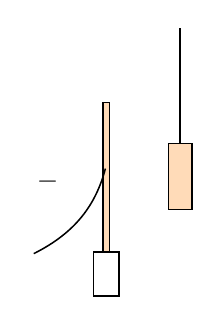
\begin{tikzpicture}[>=stealth,line width=.55pt]\draw(0,0)rectangle(.32,.56);\draw[fill=orange!28](.12,.56)rectangle(.2,2.46);\draw(1.1,3.4)--(1.1,1.94);\draw[fill=orange!28](.95,1.1)rectangle(1.25,1.94);\draw(-.76,.54)..controls(-.22,.81)and(.03,1.17)..(.15,1.62);\node[left]at(-.32,1.45){$-$};\end{tikzpicture}\end{center}Около небольшой металлической пластины, укрепленной на изолирующей подставке, подвесили на шелковой нити легкую металлическую незаряженную гильзу. Когда пластину подсоединили к клемме высоковольтного выпрямителя, подав на нее отрицательный заряд, гильза пришла в движение. Опишите движение гильзы и объясните его.
}{
\smallskip\noindent\textbf{Решение}\par
Под действием электрического поля пластины изменится распределение электронов в гильзе и произойдет ее электризация: та ее сторона, которая ближе к пластине, будет иметь положительный заряд, а противоположная сторона  — отрицательный.
Поскольку силы взаимодействия заряженных тел уменьшаются с ростом расстояния между ними, притяжение к пластине левой стороны гильзы будет сильнее отталкивания правой стороны гильзы, и гильза будет двигаться к пластине, пока не коснется ее.
В момент касания часть электронов перейдет с отрицательно заряженной пластины на гильзу, гильза приобретет отрицательный заряд и оттолкнется от одноименно заряженной пластины. Гильза отклонится вправо и зависнет в положении, в котором равнодействующая всех сил равна нулю.
}

\end{document}
